\hypertarget{ux6d77ux9f9fux7ed8ux56fe}{%
\subsection{海龟绘图}\label{ux6d77ux9f9fux7ed8ux56fe}}

在 1966 年,Seymour Papert 和 Wally Feurzig
发明了一种专门给儿童学习编程的语言------\href{https://baike.baidu.com/item/logo/4689862}{LOGO
语言},它的特色就是通过编程指挥一个小海龟(turtle)在屏幕上绘图。

海龟绘图(Turtle Graphics)后来被移植到各种高级语言中,Python 内置了
turtle 库,基本上 100\% 复制了原始的 Turtle Graphics 的所有功能。

我们来看一个指挥小海龟绘制一个长方形的简单代码:

\begin{pythoncode}
from turtle import *
width(4)
forward(200)

right(90)
pencolor('red')
forward(100)
right(90)

pencolor('green')
forward(200)
right(90)

pencolor('blue')
forward(100)
right(90)
done()
\end{pythoncode}

在命令行运行上述代码,会自动弹出一个绘图窗口,然后绘制出一个长方形:

 
 \begin{figure}[htp]
	\centering
	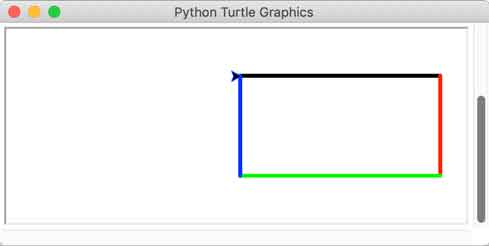
\includegraphics[width=0.6\linewidth]{fig/1249598058265600l.png}
\end{figure}


从程序代码可以看出,海龟绘图就是指挥海龟前进、转向,海龟移动的轨迹就是绘制的线条。要绘制一个长方形,只需要让海龟前进、右转
90 度,反复 4 次。

调用\texttt{width()}函数可以设置笔刷宽度,调用\texttt{pencolor()}函数可以设置颜色。更多操作请参考
\href{https://docs.python.org/3.3/library/turtle.html\#turtle-methods}{turtle
库}的说明。

绘图完成后,记得调用\texttt{done()}函数,让窗口进入消息循环,等待被关闭。否则,由于
Python 进程会立刻结束,将导致窗口被立刻关闭。

\texttt{turtle}包本身只是一个绘图库,但是配合 Python
代码,就可以绘制各种复杂的图形。例如,通过循环绘制 5 个五角星:

\begin{pythoncode}
from turtle import *

def drawStar(x, y):
    pu()
    goto(x, y)
    pd()
    
    seth(0)
    for i in range(5):
        fd(40)
        rt(144)

for x in range(0, 250, 50):
    drawStar(x, 0)

done()
\end{pythoncode}

程序执行效果如下:

 
 \begin{figure}[htp]
	\centering
	
\includegraphics[width=0.6\linewidth]{fig/1249600178485568l.png}
\end{figure}


使用递归,可以绘制出非常复杂的图形。例如,下面的代码可以绘制一棵分型树:

\begin{pythoncode}
from turtle import *
colormode(255)

lt(90)

lv = 14
l = 120
s = 45

width(lv)
r = 0
g = 0
b = 0
pencolor(r, g, b)

penup()
bk(l)
pendown()
fd(l)

def draw_tree(l, level):
    global r, g, b
    
    w = width()

    
    width(w * 3.0 / 4.0)
    
    r = r + 1
    g = g + 2
    b = b + 3
    pencolor(r % 200, g % 200, b % 200)

    l = 3.0 / 4.0 * l

    lt(s)
    fd(l)

    if level < lv:
        draw_tree(l, level + 1)
    bk(l)
    rt(2 * s)
    fd(l)

    if level < lv:
        draw_tree(l, level + 1)
    bk(l)
    lt(s)

    
    width(w)

speed("fastest")

draw_tree(l, 4)

done()
\end{pythoncode}

执行上述程序需要花费一定的时间,最后的效果如下:

 
 \begin{figure}[htp]
	\centering
	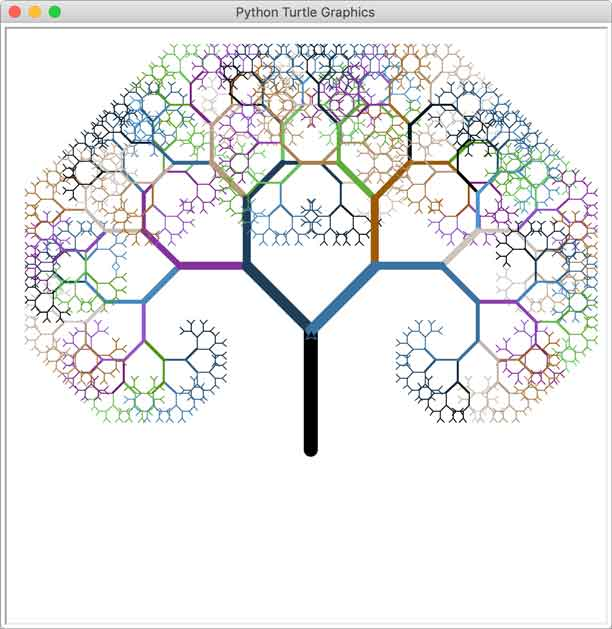
\includegraphics[width=0.6\linewidth]{fig/1249600522419392l.png}
\end{figure}


\hypertarget{ux53c2ux8003ux6e90ux7801}{%
\subsubsection{参考源码}\label{ux53c2ux8003ux6e90ux7801}}

\href{https://github.com/michaelliao/learn-python3/blob/master/samples/gui/turtle/rect.py}{rect.py}

\href{https://github.com/michaelliao/learn-python3/blob/master/samples/gui/turtle/starts.py}{starts.py}

\href{https://github.com/michaelliao/learn-python3/blob/master/samples/gui/turtle/tree.py}{tree.py}

